In this chapter we first provide an overview of traditional and latest robot programming techniques to identify common bottlenecks and issues encountered.
We end this chapter by discussing relations to this thesis.

\section{Introduction}
Robot Programming is the process of defining desired motions and associated skills so that the robot may perform them without human intervention.
Classical robot programming processes in the industry have task-specific definitions, which are generally robot-dependent, and require programming expertise.
\fig{fig:Classical robot programming process} shows the classical robot programming process, consisting of at least four phases:
The initial task definition is followed by sequencing the workcell operations.
Once the process has been validated, the robot is programmed offline using a native programming language, before it is pushed into production for regular execution.
The programmed robot can only be used for this specific task in this particular working environment.
If the task definition needs to be altered, the programming expert needs to repeat the entire programming process.
Therefore, classical robot programming processes are time-consuming and cost intensive.

\begin{figure}[ht]
	\centering
	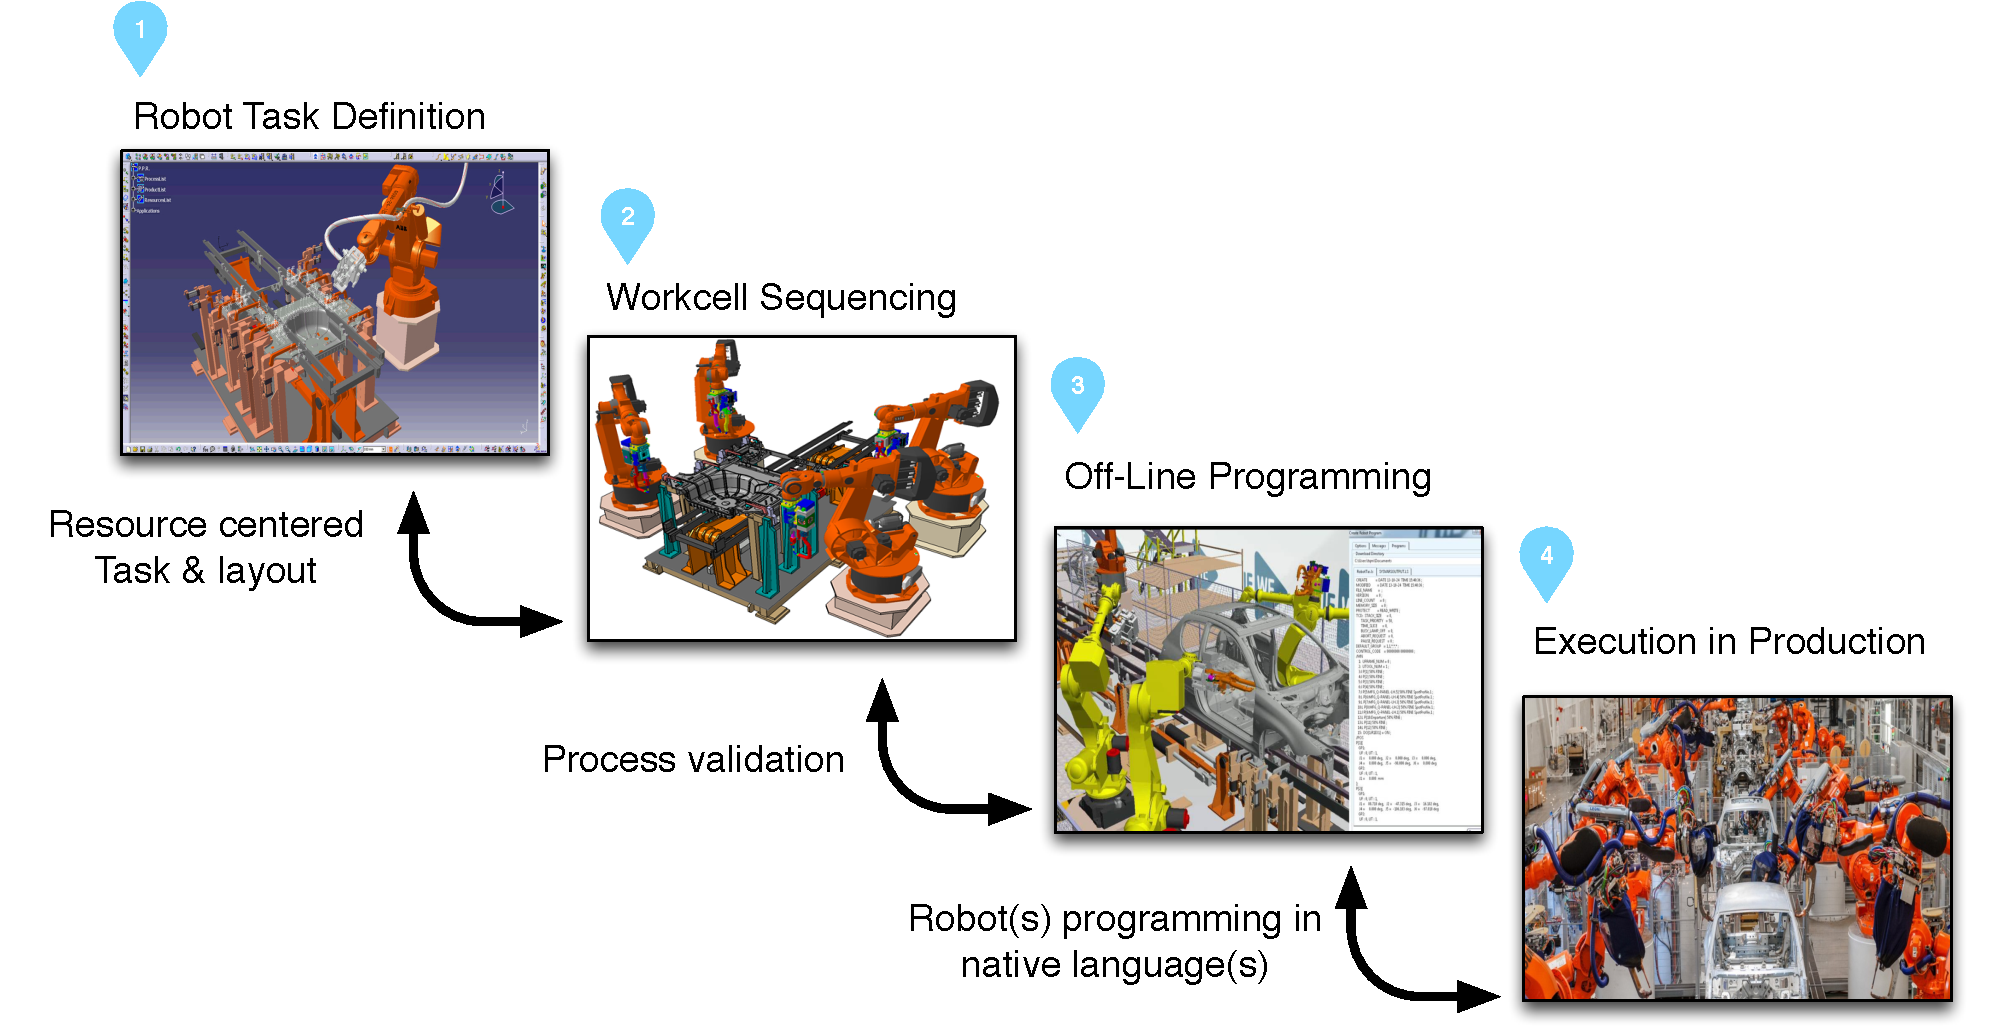
\includegraphics[width=\linewidth]{figures/manual-programming}
	\caption{Classical robot programming process}
	\label{fig:Classical robot programming process}
\end{figure}

In the past few decades, different robot programming techniques have been developed to facilitate this process. 
There are many ways to divide robot programming systems. 
\cite{lozano1983robot} divided them into three categories: 
guiding systems, where the robot's joint positions were sequentially recorded,
robot-level systems, where a programming language was used, and
task-level systems, where the task goal (\eg object positions) needs to be specified.
However, the range of programming systems was very limited at that time and examined only industrial robot programming systems.
Instead, \cite{Biggs2003} divided them into two main categories, distinguishing systems for users and for programmers:

\begin{itemize}
 \item {\textbf{Manual programming}, where the user can directly control the robot's execution code, using a text-based or a graphical system.}
 \item {\textbf{Automatic programming}, where the user does not need to write explicit code and the robot learns using a learning system, Programming by demonstration (PbD), or an instructive system.}
\end{itemize}
% - also mention software architectures which are important for any robot programming systems

% \begin{figure}[ht]
% \centering
%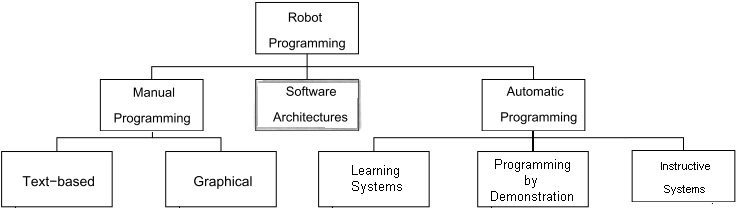
\includegraphics[width=\linewidth]{figures/Biggs2003-RobotProgramming-short}
% \caption{Robot programming categories to distinguish systems for users and programmers. (\cite{Biggs2003})}
% \label{fig:RobotProgrammingSystems}
%\end{figure} 

Inspired by \cite{Biggs2003}, we created a new robot programming overview (\fig{fig:RobotProgrammingOverview}) involving techniques that have been applied in most recent research.
Even though many state of the art systems use a combination of techniques, such as Deep Reinforcement Learning (\cite{arulkumaran2017brief}) or PbD for Reinforcement Learning (\cite{hester2017learning}), it makes sense to differentiate them by their key attributes, which we identified as follows: 
%control over the robot code, learning data, and end-user involvement.
\begin{itemize}
	\item \textbf{Control over the robot behaviour:} if the robot behaviour code is directly entered and how it is generated (text-based or visual programming) and if the code directly encodes the robot's executed behaviour (manual or automatic programming)
	\item \textbf{Learning data:} for automated programming systems the robot learns from data and we differentiate how it is acquired (provided by the teacher vs by self-exploration), and what type it is (\eg positive vs negative examples, labelled)
	\item \textbf{End-user involvement:} the level that the end-user is involved in the programming process ranging from writing code manually, providing data or continuous feedback during the learning process to defining reward functions.
\end{itemize}

%From an end-user programming perspective, it is useful to assign different levels of teacher involvement in the programming process and an estimation of the programming time required.
In the following sections we will give a brief overview of the different programming systems by first distinguishing between the user's control over the robot behaviour, \ie manual (\sect{subsec:Manual Programming Systems}) and automatic (\sect{subsec:Automatic Programming Systems}) programming.
For manual programming, we compare text-based (\sect{sssec:Text-based Systems}) and graphical (\sect{sssec:Graphical systems}) systems.
For automatic programming, we differentiate those that learn from unbiased and biased data, \ie machine learning systems (\sect{sssec:Learning Systems}) vs programming by demonstration (\sect{sssec:PbD}).
Finally, we will discuss different levels of end-user involvement and their interaction modalities (\sect{sssec:End-User Involvement}).

%\begin{table}[ht]
%\begin{center}
%\begin{tabular}{r|c|c}
%Programming Techniques & by Exploration \newline (unguided) & by Demonstration \newline (guided)\\ \hline
%Classification & \checkmark & \checkmark \cite{saunders2006teaching,hovland1996skill,rybski1999interactive} \\
%Regression & \checkmark & \checkmark \cite{atkeson1997locally,pomerleau1991efficient} \\
%Reinforcement Learning & \checkmark & \checkmark (System models) \cite{atkeson1997robot,smart2002effective,abbeel2004apprenticeship}.\\
% Plans & \checkmark & \checkmark \cite{kuniyoshi1994learning,ekvall2008robot} \\
% \hline
%Human-Robot Interaction & & \\ \hline
% touch & \checkmark (learning by poking) & \checkmark \\
% vision & \checkmark & \checkmark \\ 
% voice & n/a & \checkmark (instructive, create sequence by voice) \\
%\end{tabular}
%\end{center}
%\label{tab:Programming Overview}
%\end{table}


\section{Manual Programming Systems}\label{subsec:Manual Programming Systems}
In manual programming systems users have direct control over the robot code
and often require expert knowledge in a programming language. % and a good understanding of the program flow.
There exist a variety of tools to make programming, as well as testing and debugging, easier such as IDEs, spreadsheets, macros, \etc 
There are two types of manual programming: text-based programming, where the code is written manually in a chosen programming language (python, C++, java, \etc) and graphical programming, where the code structure is created with the help of a graphical interface (\eg Flowcharts). 

\subsection{Text-based Systems}\label{sssec:Text-based Systems}
Text-based systems are one of the most common methods and use a traditional programming approach. 
Depending on the type of language used, the user performs programming in either controller-specific languages, where the robot-specific machine language consists of simple commands, \eg the KUKA Robot Language (\cite{braumann2011parametric,muhe2010reverse}) shown in \fig{fig:Kuka},
% RAPID a high-level programming language to control ABB robots
generic procedural languages, where multi-purpose languages such as C++ that have been extended with classes to provide simple access to common robot specific functions ({\eg Lego}), or behaviour-based languages that specify how the robot should react to different conditions (\eg Haskell). 
There has been a trend to move from low-level command-based languages towards more intelligent programming systems with high-level languages that provide more support to the user and reduce the programming workload.
However, text-based systems still require trained users with programming knowledge and are more likely to be used by robot developers than end-users.

\clearpage
\begin{sidewaysfigure}[!h]
	\centering
	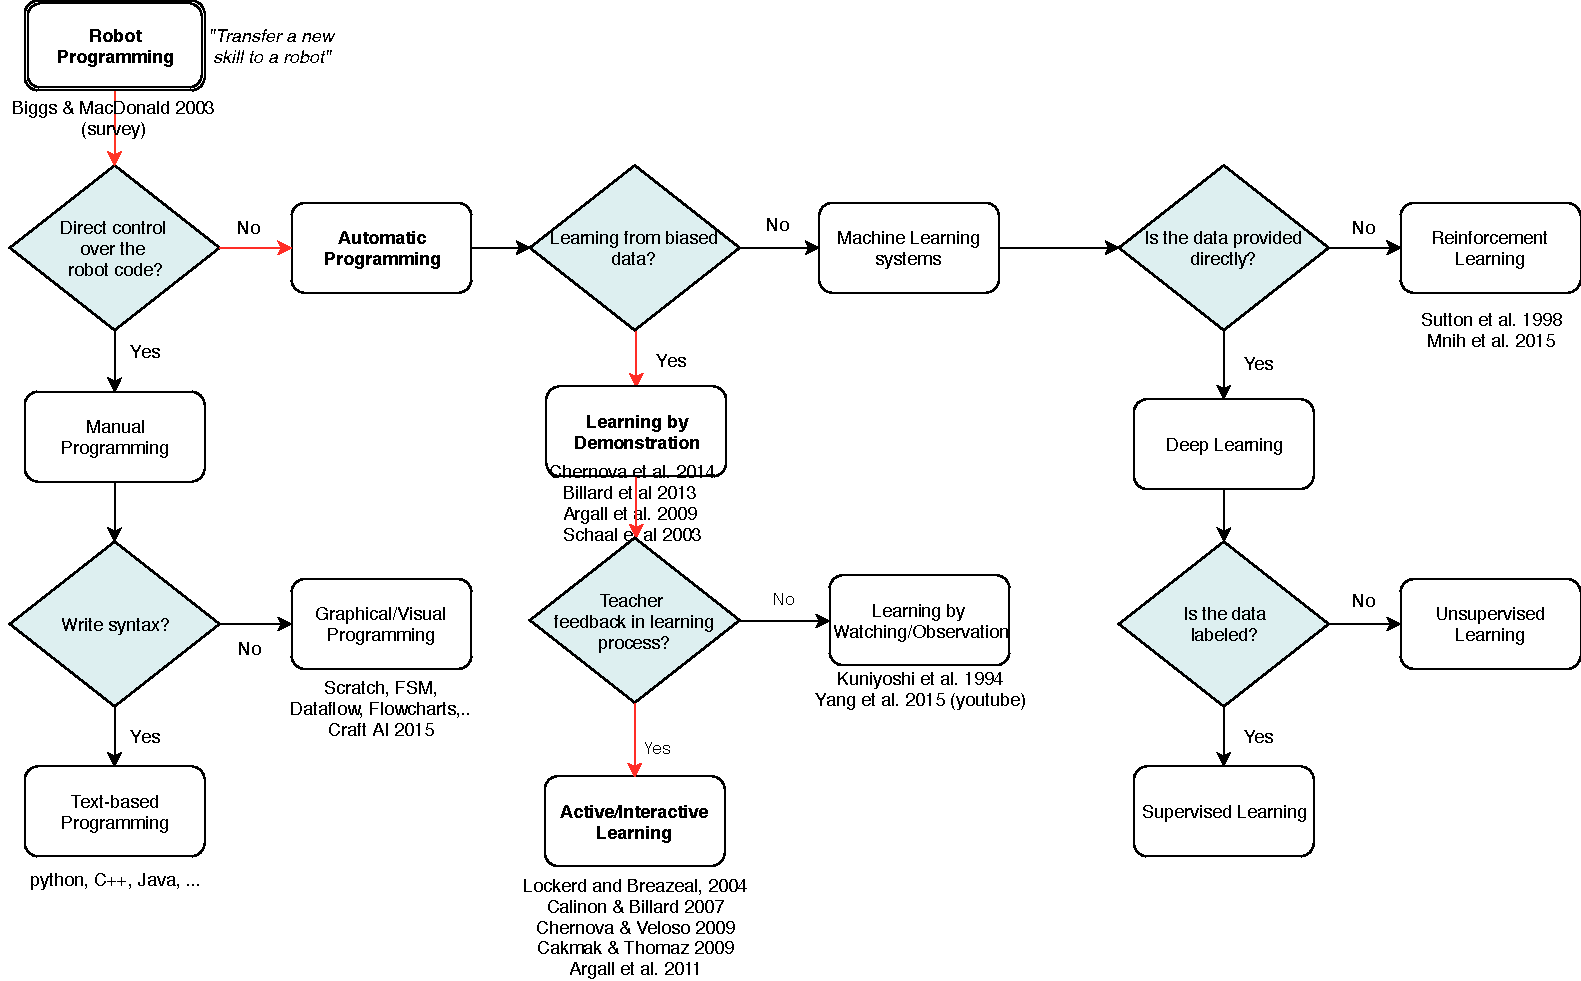
\includegraphics[width=0.9\linewidth]{figures/RobotProgrammingOverview}
	\caption{Overview of Robot Programming methods.}
	\label{fig:RobotProgrammingOverview}
\end{sidewaysfigure}
\clearpage

\subsection{Graphical Systems}\label{sssec:Graphical systems}
Graphical (or icon-based) systems use a graph, flow-chart or diagram view where users manually specify actions and program flow.
The graphical icons correspond directly to the program statements.
\cite{lego2003} and \cite{bischoff2002morpha} produced graphical systems using a flow-chart approach, where the robot's behaviour can be configured by arranging low-level actions in a sequence (\fig{fig:lego-mindstorm}).
Similarly, Scratch (\cite{majed2014learn}) is a block-based visual programming language to allow children with no programming experience to learn development in an intuitive way for animations and interactive applications (\fig{fig:scratch-interface}).
\cite{huang2017code3} created a system for programming mobile manipulator robots with a drag-and-drop interface as a high-level programming component.
For all of these systems, the user has direct control over the programmed behaviour, thus increasing their programming effort.
%They are typically easy to use and generally used for robot applications rather than system programming. 
\section{Automatic Programming Systems}\label{subsec:Automatic Programming Systems}
Automatic programming systems relate to robots that can learn from data and generate their behaviour, known as a \textit{policy}, from data provided as input to the system.
Unlike manual programming, the end-user does not need to sequence robot code and does not have direct control over the robot's executed behaviour.

\subsection{Deriving a policy}\label{subsec:Deriving a policy}
%Our focus is on the former, learning low-level trajectories that can be generalised.
%The latter will then be taken over by automated planning techniques.
The problem of learning a behaviour or \textit{skill} can be considered as learning a function that maps a world state to an action.
In real-world applications, states can only be partially observed due to restricted sensor availability.
Hence, we assume that the robot learner has access to the observed state $Z$ instead.
A function $\pi : Z \rightarrow A$, referred to as a \textit{policy}, allows the robot to select actions from an action domain $A$, given observations of the world state.
States can either be represented in a discrete way (\textit{``object on the table"} or \textit{``robot holding object"}) or in a continuous way \eg using the robot's end effector pose (Table \ref{tab:representations}).

Once the training data has been acquired, the robot learner needs to derive a policy $\pi : Z \rightarrow A$, a state-action mapping from the observed state to the action domain representing the desired behaviour.
The most efficient policy derivation techniques approximate the state-action mapping from as few training data as possible.
\cite{chernova2014robot} give an overview of state of the art techniques.

\begin{table}[ht]
	\centering
	\begin{tabular}{r|ll}
		& Continuous representation & Discrete representation\\ \hline
		Position & (x,y,z) coordinates & table \\
		Orientation & ($\theta_x,\theta_y,\theta_z$) & straight/upright \\
		Colour & (r,g,b) & red, yellow, green\\
		Spatial relation & (x,y,z) distance vector & left/right/front/behind of 
	\end{tabular}
\caption{State representations: continuous vs discrete}
\label{tab:representations}
\end{table}

A policy can describe either a low-level skill (\ie a motion trajectory) or a high-level task (\ie symbolic encoding).
Low-level representations focus on learning generalised trajectories, high-level representations focus on learning a sequence of motion elements (primitives) (\cite{peppoloni2014ros}). 
In the following we will give an overview of both techniques.

\clearpage
\begin{figure}[!h]
	\centering
	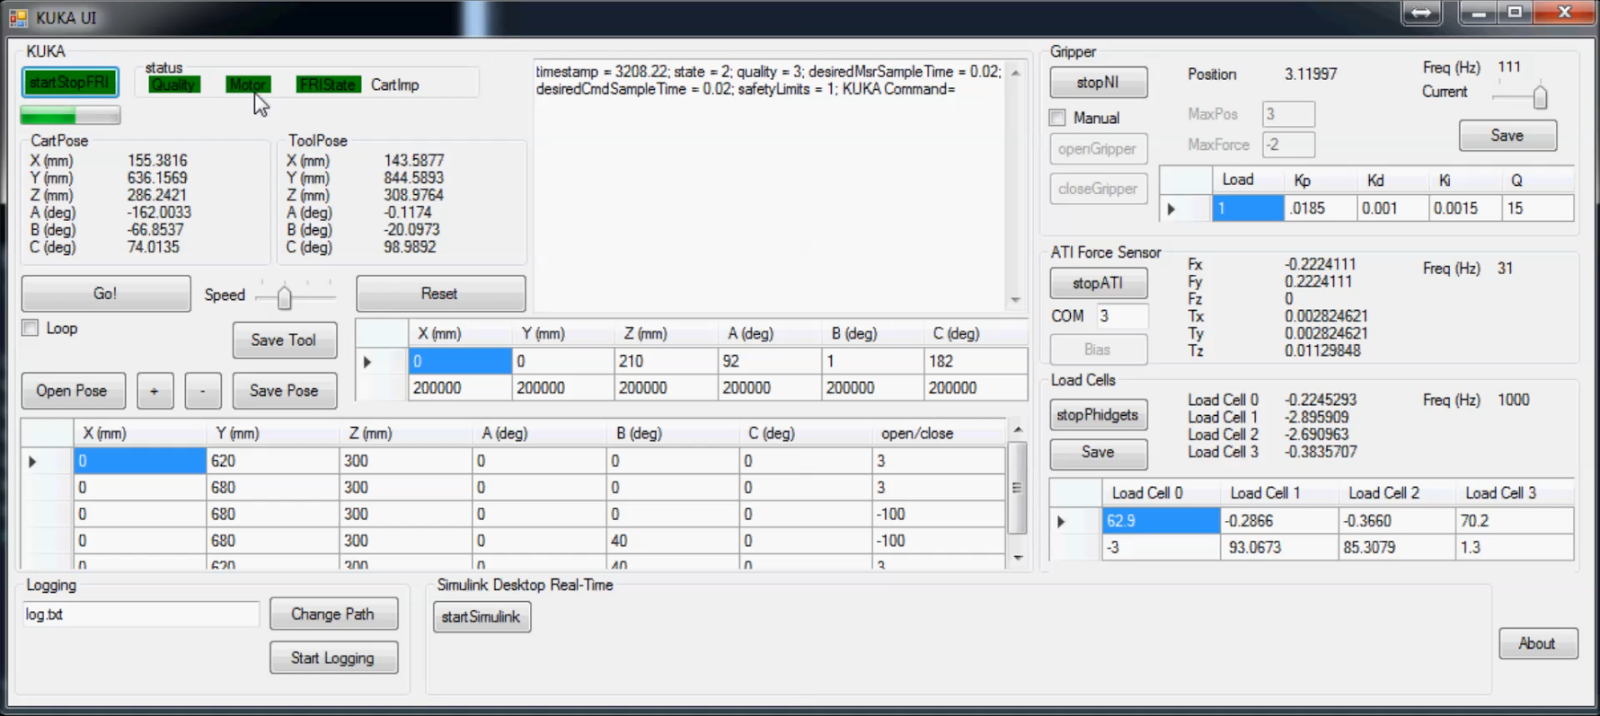
\includegraphics[width=0.99\linewidth]{figures/kuka-interface2}
	\caption{KUKA Robotics graphical user interface (\cite{abdeetedal2017kuka})}
	\label{fig:Kuka}
\end{figure} 
\begin{figure}[!h]
	\centering
	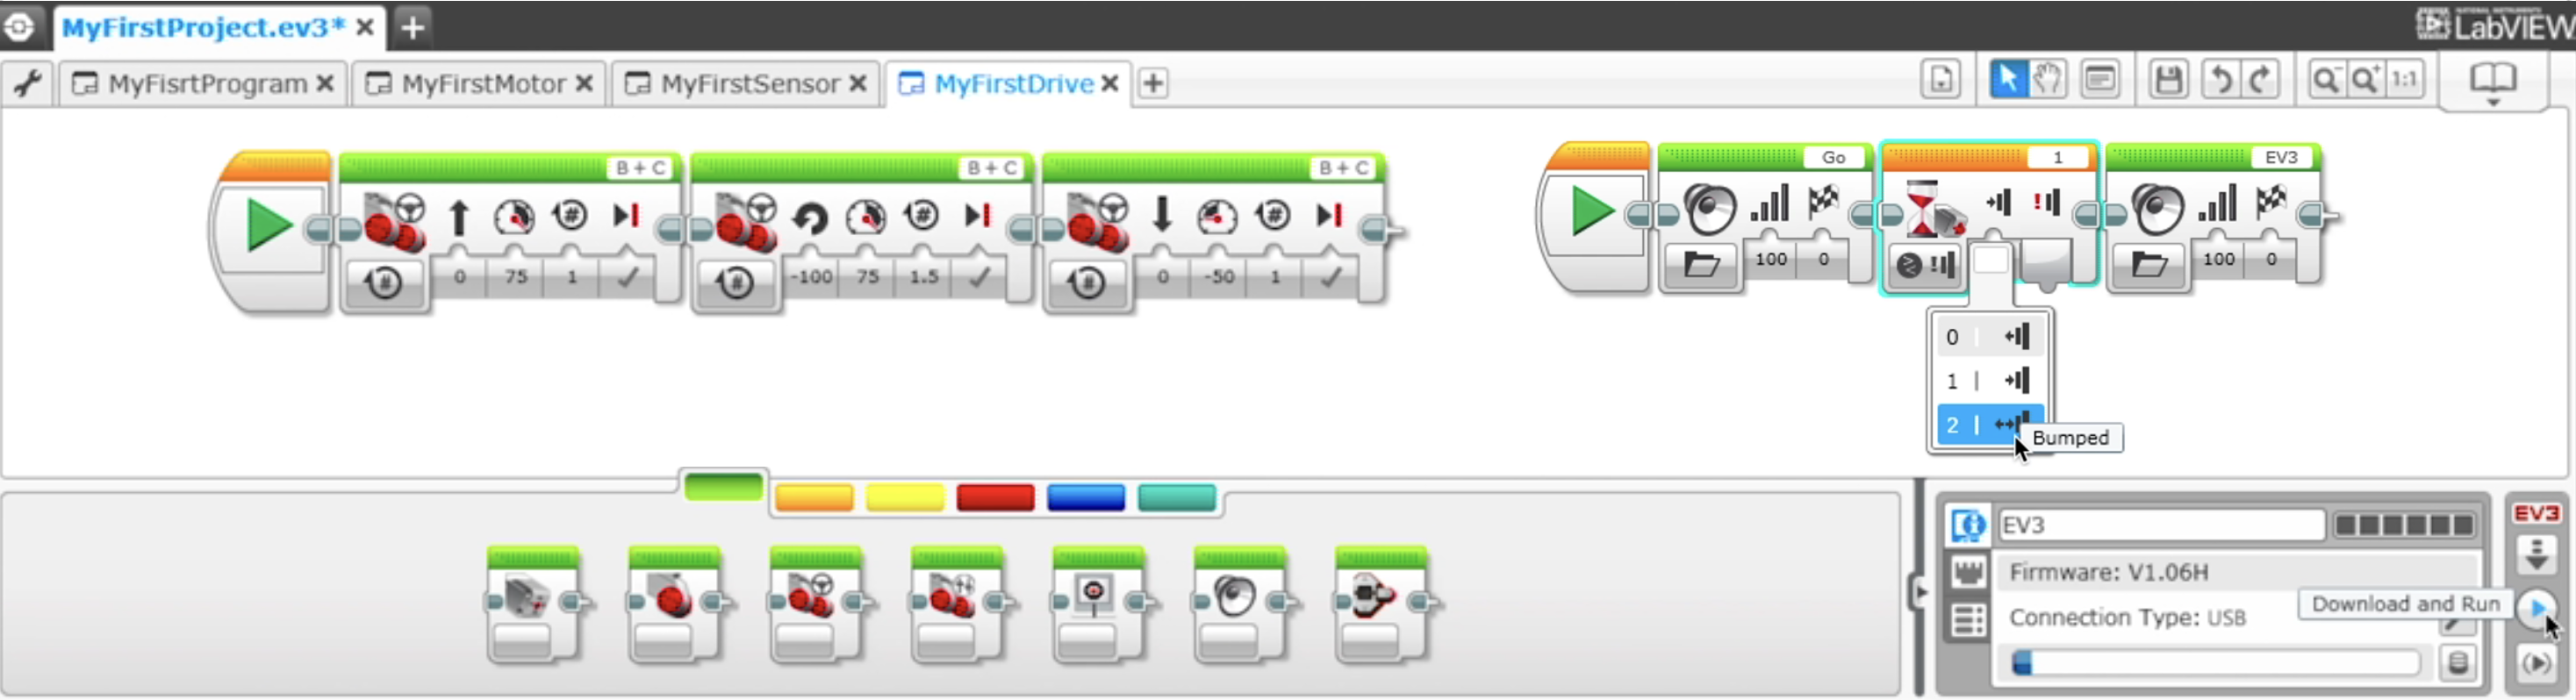
\includegraphics[width=\linewidth]{figures/lego-mindstorm2}
	\caption{Lego Mindstorms EV3 icon-based interface (\cite{lego2003})}
	\label{fig:lego-mindstorm}
\end{figure} 
\begin{figure}[!h]
	\centering
	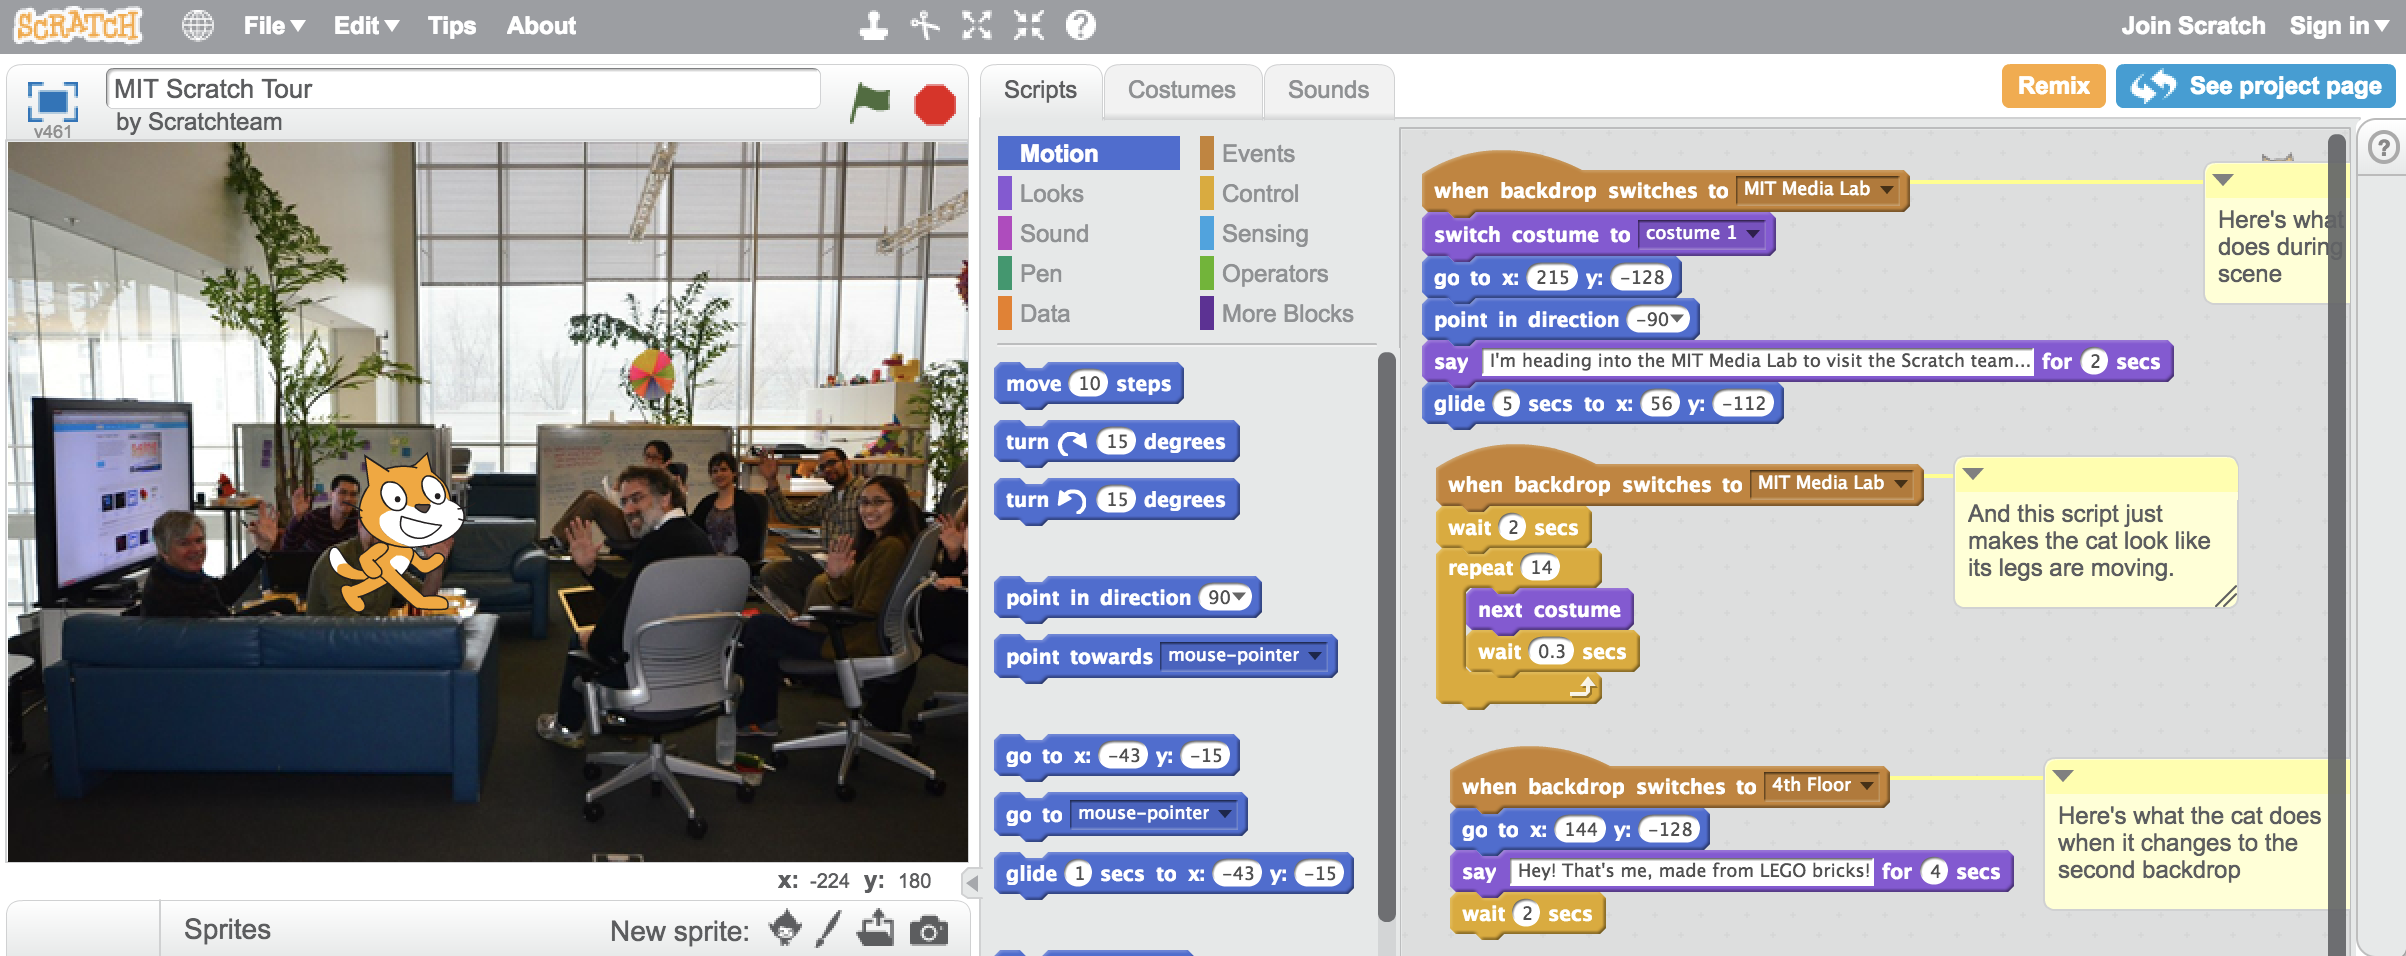
\includegraphics[width=\linewidth]{figures/scratch-interface}
	\caption{Scratch: block-based visual programming language (\cite{majed2014learn})}
	\label{fig:scratch-interface}
\end{figure} 
\clearpage
\subsubsection{Low-level skill learning}\label{ssec:lowlevel}
In the literature low-level actions have been referred to as \textit{skill, motor skill, primitive action,} or \textit{low-level motion} (\cite{chernova2014robot}).
Generalisable low-level actions can be learned by recording joint angle trajectories using GMM (\cite{billard2008robot}), using keyframe-based learning (\cite{akgun2012keyframe}), or using Dynamic Movement Primitives (DMP) (\cite{pastor2009learning}), which consist of differential equations that can create a smooth trajectory to a new goal point.

For instance, in keyframe-based learning, demonstrations are provided by kinesthetically manipulating the robot's arm and recording a series of end-effector positions (or \textit{keyframes}). 
An end-effector pose can be relative to the robot's base or to a landmark previously detected by the robot.
Landmarks are only known to the robot after a table top detection step has been performed.

\subsubsection{High-level task learning}\label{ssec:highlevel}
For learning high-level tasks it is assumed that a set of low-level primitive actions is preprogrammed into the robot. 
\cite{she2014teaching} teaches the robot new high-level actions by instructing the robot a sequence of lower-level actions.
Rather than representing the new action as an action sequence, it is modelled by their desired goal states calculated as:
$A_i(c_1 \dots c_k) = (S_e - S_e \cap S_b) \cup p_{grip}$ where $c_i$ are objects in the scene, $S_b$ and $S_e$ are the states at the beginning and end of the instruction and $p_{grip} = \{open, close\}$ is the gripper status at the end of instruction.
As the work uses the blocks world domain with a single object type (`block'), an operator for the new high-level action can be inferred easily. Preconditions and effects for the domain are already specified in advance.

\subsection{Learning from data} \label{subsec:Gathering data}
There are different ways to gather data depending on the amount provided at a time (incremental vs. batch learning) and the different interaction modalities (voice, vision, and touch) to transfer the data to the robot.
The robot can learn from data that is directly related to the desired behaviour and has been selected by a teacher (\eg learn from optimal teacher demonstrations), which we refer to as learning from \textit{biased} data.
If the robot learns from data that is not directly related to its executed behaviour (\eg from trial and error), we refer to it as learning from \textit{unbiased} data.
Thus, we differentiate automatic programming systems between Machine Learning systems (\sect{sssec:Learning Systems}), where the robot learns from \textit{unbiased} data, and Programming by Demonstration (\sect{sssec:PbD}), where the robot learns from \textit{biased} data.
Many approaches derive a policy using vision by having the robot learn from image or video data or by observing a human teacher (\cite{kuniyoshi1994learning}).
RL systems gather data autonomously by exploring the environment where the robot repetitively executes its actions and learns from the observed state changes.
Recent approaches have combined these approaches to improve performance and accelerate the learning process, \eg Deep Reinforcement Learning (\cite{arulkumaran2017brief}) or PbD for Reinforcement Learning (\cite{hester2017learning}).
As this is beyond the scope of this thesis, we will give a brief overview of the main two approaches and leave their discussion for future work.


\subsection{Machine Learning Systems}\label{sssec:Learning Systems}
Machine Learning (ML) systems use inductive inference to create a program by taking examples provided by the user or from self-exploration of the robot. 
The goal of these systems is to construct programs that allow the robot to automatically improve its performance with increasing amounts of data. 
Even though ML algorithms have been around since the 1980s, it has only become popular in the past few decades. 
The rise of the internet led to big data, improved knowledge sharing, and advances in techniques to process and store data efficiently triggered a wave of new ML techniques.
%Developments in various research areas such as computer vision have impacted the field of robotics.
Recent applications of ML in robotics\footnote{http://techemergence.com/machine-learning-in-robotics/} include research areas such as computer vision (or ``robot vision'') for the identification and sorting of objects (\cite{stager2013computer}) and imitation learning to learn action plans from watching unconstrained videos (\cite{Yang2015}).

We can differentiate between how the data is acquired: 
In Deep Learning (DL), data is provided directly to the robot in either labelled (supervised learning) or unlabelled format (unsupervised learning).
In Reinforcement Learning (RL), the robot acquires data by self-exploration of its environment where the robot enters different states depending on the actions it takes (\fig{fig:ml-types}).
DL systems (\cite{schmidhuber2015deep}) generally use artificial neural networks (NN) which require large amounts of data to learn the desired behaviour.
Techniques are divided into supervised (\eg Classification, Regression) and unsupervised (\eg Clustering) learning, using labelled and unlabelled data respectively.
%\cite{billard2001robust} used NN to learn the motion of a human arm in 3D.

RL systems (\cite{sutton1998reinforcement,kaelbling1996reinforcement,gosavi2009reinforcement}) learn from data acquired from self-exploration of the environment. 
The robot uses a reward function to learn its policy, while taking random actions and refines it by updating expected rewards with observed outcomes.
However, setting up the states, actions, and policy is often difficult and usually requires a robotics expert.
\cite{kober2013reinforcement} provides a survey of work in RL to generate behaviour for robots and highlights the main challenges that are faced.
Since the robot has to explore many states before it can learn the correct behaviour, RL systems usually take hundred or thousands of training examples.
To accelerate the learning and reduce the amount of exploration required, recent work includes teacher demonstrations with RL solutions (\cite{martinez2017relational,hester2017learning}).
%There are two main classes of RL approaches, namely \textit{model-based} (\cite{polydoros2017survey}) and \textit{model-free }(\cite{kober2013reinforcement}) methods, differentiating between whether a model of the interactions between the robot and the environment is used, or whether it learns from samples.
%While model-based methods converge faster to the optimal solution, an accurate model is not always available and can impact the learning process.
%Model-free methods require the robot to learn from samples, resulting in a slow convergence to the optimal solution.

%In real world scenarios robots require teacher input to learn behaviours efficiently. 
%\todo{Similar to our work: \cite{martinez2017relational}}

%Inverse reinforcement learning (\cite{abbeel2011inverse}) is a supervised RL mode where the learner tries to acquire the reward function from demonstrated behaviours.
%This is can also be considered a learning from demonstration approach.

\begin{figure}[ht]
	\centering
	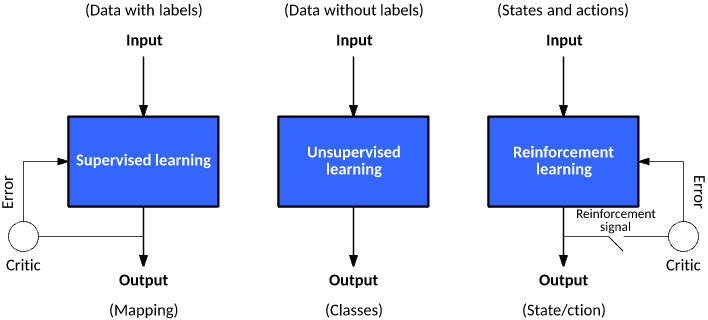
\includegraphics[width=\linewidth]{figures/ml-techniques}
	\caption{Types of Machine learning: Deep learning (supervised and unsupervised learning) and Reinforcement learning (\cite{jones2017models})}
	\label{fig:ml-types}
\end{figure}

\subsection{Programming by Demonstration}\label{sssec:PbD}
Programming by Demonstration (PbD) (\cite{billard2016learning,argall2009survey}), also known as Learning from Demonstration or Imitation Learning, describes various techniques where the robot learns new behaviours from teacher demonstrations.
It provides an intuitive medium to allow non-roboticists to easily communicate skills to robots.
Unlike ML solutions, the provided data is generally sparse and directly correlated with the robots executed behaviour, \eg human teachers providing optimal demonstrations.
The underlying concept is for the robot to learn a new skill from these demonstrations, thus reducing the complexity of the search space and accelerating learning.
As the teacher selectively provides demonstrations that the robot should learn from, we refer to this as \textit{biased} data.

%``Programming by demonstration (PbD) has become a central topic of robotics and spans across general research areas such as human-robot interaction, machine learning, machine vision and motor control" (\cite{billard2008robot}).

%PbD systems have been used in the industry for creating assembly programs. 
%It offers a framework for service robotics applications, independent of the robot platform, and reduces the overhead of reprogramming the robot for different tasks.
%In recent years there has been significant work in PbD to move from pure imitation to intelligent systems that learn flexible task executions. 
%PbD systems may learn task descriptions from interpreted data to adapt the learned task to changing environments.

\subsubsection{Providing demonstrations}
There exist various techniques for providing demonstrations.
\cite{argall2009survey} define four categories by differentiating between the choice of the demonstrator (human or robot) and who executes the demonstration:
The teacher could demonstrate either using their own hands (\textit{shadowing} or \textit{external observation}), by wearing sensors (\textit{sensors on teacher}), or by moving the robot's joints directly (\textit{kinesthetic teaching} or \textit{teleoperation}).
If the demonstration is not recorded directly on the robot's joints, the demonstrated trajectory has to be extracted and mapped to the robot's joints.
This is known as the correspondence problem (\cite{nehaniv2002correspondence}), which describes the difference of humans and robots regarding their sensing abilities and physical embodiment.
If the robot joints are recorded directly from the demonstration by teleoperation or kinesthetic teaching, this problem is eliminated (\cite{chernova2014robot}).
Previous work showed that kinesthetic guidance can be problematic in narrow spaces (\cite{wrede2013user}) or if the objects are large or dangerous to operate (\cite{chernova2014robot}).
However, comparing kinesthetic teaching with teleoperation showed that kinesthetic teaching produced better results in terms of efficiency, effectiveness (success and error rate), and usability \cite{fischer2016comparison,chernova2014robot,akgun2011robot}.


%%%%% Gathering demonstrations
The user can choose to provide positive or negative examples (\cite{grollman2012robot}), to allow the robot to learn more efficiently by reducing the search space for possible solutions.
Positive examples are demonstration data showing what the robot should do and what it can learn directly from. %, \ie where an action changes predicates.
Negative examples are what the robot should avoid and help to generalise faster by eliminating bad solutions from the search space. %, \ie when an action fails because its preconditions are not satisfied.
\cite{walsh2010efficient} noted that negative examples are highly uninformative as the learner cannot easily determine the reason for the failure, while positive examples provide very useful information because a superset of the literals that belong to the action preconditions is identified.

\subsubsection{Interaction modalities}
Natural language is the most intuitive way for humans to communicate instructions but may need some form of clarification and learning system in order to work efficiently. 
Instructive systems that use voice recognition to command robots to carry out tasks provide the user with a high-level control to program the action sequence by commanding sub-actions that have already been programmed into the robot (Forbes et al. 2015).
%Instructive systems use voice recognition to command robots to carry out tasks while performing a demonstration.
Voice recognition is also used in PbD systems during demonstrations to activate in-built actions such as opening gripper or save end-effector poses (\cite{alexandrova2014robot}).
%The teacher can also demonstrate the action using their own hands, while the robot observes the motion (\cite{kuniyoshi1994learning}).
Gestures can be used to direct the attention of the robot for indicating objects in a scene to which the instructions apply.
Demonstrations can also be provided by kinesthetically moving the robot's joints, allowing the robot to go through the action execution.
A multi-modal communication including information from vision, gesture and voice sources can be used to clarify instructions to the robot, for example mentioning ``that table" and gesturing the relevant object.
\cite{profanter2015analysis} evaluated four input modalities (touch, gesture, speech, 3D tracking device) and showed that users preferred touch and gesture input and that speech input was the least preferred modality.

%Programming by demonstration is an approach to learn this policy from demonstration data, known as \textit{examples}.
% ``Examples are sequences of state-action pairs that are recorded during the teacher's demonstration of the desired robot behaviour." \cite{argall2009survey} 
%Unlike learning techniques in reinforcement learning, PbD is aimed at learning from correct examples only.
%Thus, PbD can be seen as a subset of Supervised Learning, as the agent is presented with labelled training data and tries to learn an approximation of the function, which produced the data (\cite{argall2009survey}).


%In contrast to reinforcement learning techniques, where the policy is learned from arbitrarily positive and negative experience, PbD approaches derive the policy from a dataset of selected examples.
%The robot derives a policy in various ways (\sect{subsec:Deriving a policy}). 

\subsubsection{Interactive Policy Refinement Techniques}\label{subsec:Other RP Methods}
As human demonstrations are often noisy or suboptimal, interactive policy refinement techniques can be used.
The robot can learn from observation data provided by the teacher (Learning by Observation), by self-exploration using a defined reward function (Learning by Exploration), or by interactive teaching from continuous feedback (Active Learning). 
Learning by exploration allows the robot to refine the policy on its own and can be combined with teacher critique. 

%\subsubsection{Learning by Exploration}\label{sssec:LbExploration}
%- the robot acquires data from interaction with its environment
%- need a reward function which allows him to learn from the data
%1. Reinforcement learning (\cite{sutton1998reinforcement}, \cite{mnih2015human})
% - reward function can be specified by the user, robot learns policy by self-exploration
% 2. Inverse reinforcement learning (\cite{abbeel2004apprenticeship})
% - robot is given teacher demonstrations and learns reward function
For active, or \textit{interactive}, learning, the teacher provides the robot with initial data, observes its performance when executing the learned action and then provides further feedback (\cite{nicolescu2003natural,calinon2007active,calinon2007incremental}).
%They implement systems, which actively involve the teacher in the robot's learning process, by providing human guidance to a humanoid robot. 
The robot first observes the demonstration performed by the teacher, who is wearing motion sensors. 
When it tries to reproduce the action, the teacher can refine the movement by physically moving its limbs.
In \cite{nicolescu2003natural} the robot refines the learned skill using feedback cues provided by the teacher and by inserting or removing behaviours from the network of abstract behaviours.
Learning tasks from interactions with a teacher is also known as \textit{Interactive Task Learning} (\cite{laird2017interactive}), where the goal is to learn through natural communication and to improve performance via instruction, demonstration, and feedback. 
The robot can also request feedback from the teacher when encountering problems during action execution (\cite{cakmak2012aaai,abdo2013learning,martinez2017relational}).
Other policy refinement approaches allow the teacher to modify the taught actions using a graphical interface, therefore minimising the number of demonstrations required (\cite{alexandrova2015roboflow,paxton2017costar,perzylo2016intuitive,stenmark2017simplified}).

%\cite{martinez2017relational} propose a relational RL solution with guided demonstrations where the robot requests for help from the human teacher to reduce the learning time.
%However, demonstrations are only requested if they yield significant improvements as the teacher's time is considered more valuable than the robot's time.

%ITL: The central challenge consists of ``converting externally specified descriptions of a task into internal representations that are incrementally integrated with existing knowledge".
%The authors mention that PbD simplifies the programming process but is generally limited by the types of tasks being taught due to the restricted knowledge that can be transferred through demonstrations.

%\todo{check Imitation learning survey}

%\subsubsection{Robot feedback}
%Robot feedback is important to provide the teacher with enough information about what to demonstrate to the robot.
%Reasons such as wrong preconditions or missing action effects can lead to failures.
%Failures can be explained using excuses \cite{?}
%Benchmark: \cite{martinez2017relational} uses 3 examples from Planning competitions

\section{End-user Involvement}\label{sssec:End-User Involvement}
There are different levels of end-user involvement in robot programming, such as writing and organising the execution code, providing biased or unbiased data, and defining reward functions. 
Inspired by \cite{kormushev2013reinforcement} who compared robot teaching approaches,
%by computational complexity with difficulty for the teacher.
Table \ref{tab:enduserinvolvement} shows an overview of user involvement tasks, estimated difficulty, data and time required to teach the robot.
We consider five categories from `high', `moderately high', `medium', `moderately low', and `low'.
%In this case we consider experts as users who have received formal training or experience in the stated robot programming method, \eg programming languages or RL/DL-related concepts.

%\begin{figure}[ht]
%	\centering
%	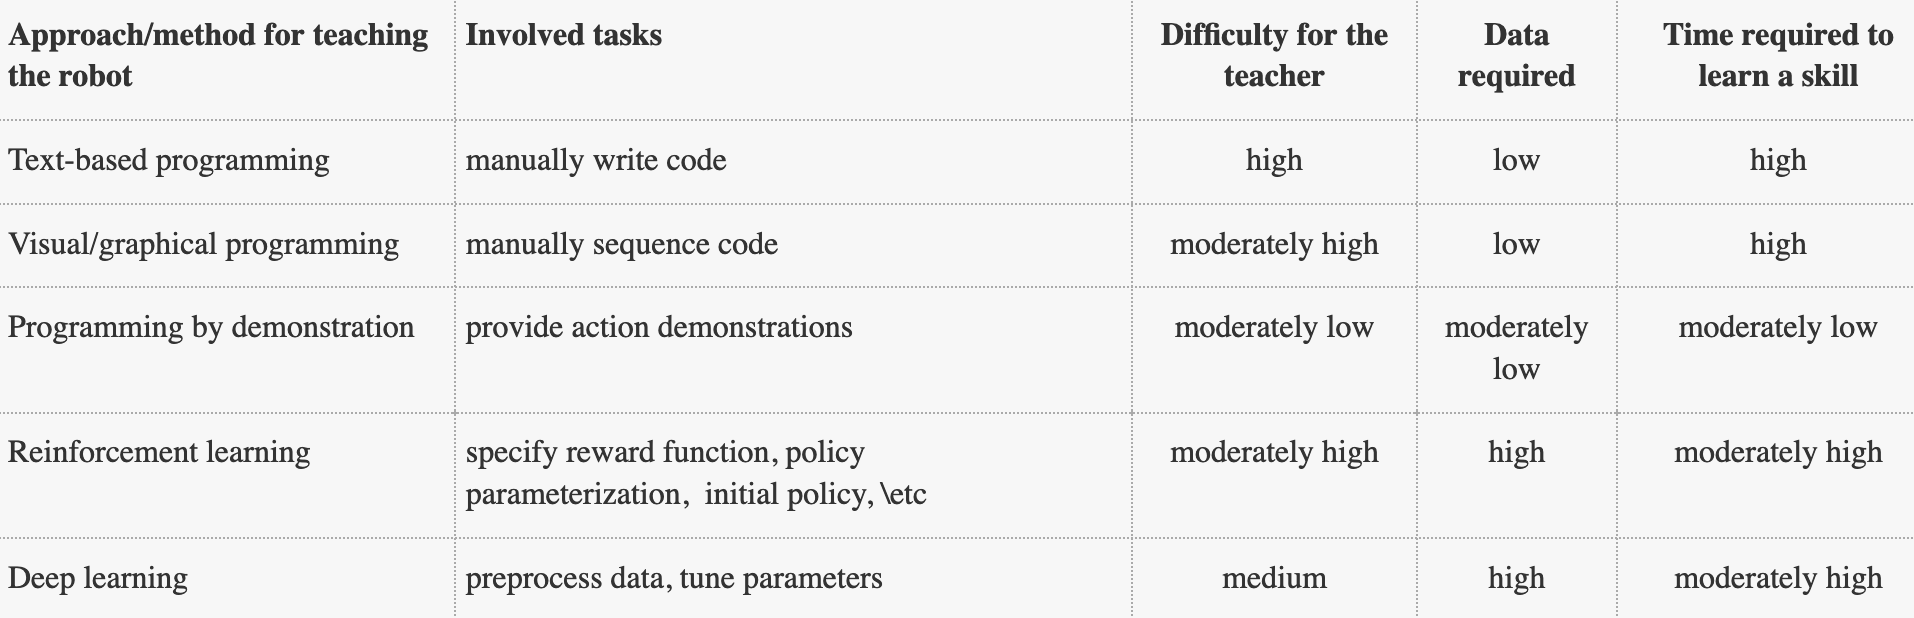
\includegraphics[width=\linewidth]{figures/robot-programming-comparison}
%	\caption{End-user involvement for common robot programming approaches}
%	\label{tab:enduserinvolvement}
%\end{figure}

\begin{table}[h]
	\begin{tabular}{@{}l@{\hskip1.5pt}l@{\hskip1pt}c@{\hskip1pt}c@{\hskip1pt}c}
		\noindent\begin{tabular}{@{}l}
			\textbf{Programming}\\
			\textbf{approach}
		\end{tabular}  & \textbf{Involved tasks}& 
		\begin{tabular}{c}
			\textbf{Difficulty}\\
			\textbf{for the teacher}
		\end{tabular}  & 
		\begin{tabular}{c}
			\textbf{Data}\\
			\textbf{required}
		\end{tabular}  &
		 \begin{tabular}{c}
			\textbf{Time required}\\
			\textbf{to learn skill}
		\end{tabular} \\ \hline
		Text-based    & manually write code    & high& low & high\\ \hline
		Visual/graphical  & manually sequence code & 
		\noindent\begin{tabular}{@{}c}
			{moderately}\\
			{high}
		\end{tabular}   & low & high\\ \hline
		\noindent\begin{tabular}{@{}l}
			{Programming}\\
			{by demonstration}
		\end{tabular}  & provide demonstrations  & 
		\noindent\begin{tabular}{@{}c}
		{moderately}\\
		{low}
		\end{tabular} & 
			\noindent\begin{tabular}{@{}c}
			{moderately}\\
			{low}
		\end{tabular}    & 
			\noindent\begin{tabular}{@{}c}
			{moderately}\\
			{low}
		\end{tabular}     \\ \hline
		\noindent\begin{tabular}{@{}l}
			{Reinforcement}\\
			{learning}
		\end{tabular}  &
		\noindent\begin{tabular}{@{}l}
			specify reward function, \\
			policy parameterization,  \\
			initial policy, \etc \\
		\end{tabular} 
		& 
		\noindent\begin{tabular}{@{}c}
			{moderately}\\
			{high}
		\end{tabular} & high & 
		\noindent\begin{tabular}{@{}c}
			{moderately}\\
			{high}
		\end{tabular}   \\ \hline
		Deep learning   & 
		\noindent\begin{tabular}{@{}l}
			preprocess data,\\ 
			tune parameters \\
		\end{tabular}   & medium   & high& 
	\noindent\begin{tabular}{@{}c}
	{moderately}\\
	{high}
\end{tabular} 
	\end{tabular}
\caption{End-user involvement for common robot programming approaches}
\label{tab:enduserinvolvement}
\end{table}
%
%\begin{table}[h]
%	\centering
%	\begin{tabular}{llcc}
%		 \textbf{Programming method} & \begin{tabular}{@{}l@{}}\textbf{End-user task} \\ \textbf{required}\end{tabular} & \begin{tabular}{@{}l@{}}\textbf{Effort} \\ \textbf{required}\end{tabular} & \begin{tabular}{@{}l@{}}\textbf{Expertise} \\ \textbf{required}\end{tabular} \\ \hline
%		Write code manually & Text-based programming & high & yes \\
%		Organise code sequence & Visual programming & moderately high & no \\
%		\begin{tabular}{@{}l@{}}Provide complete data, \\ Tune parameters \end{tabular} & Deep learning (DL) & moderate & yes \\
%		Provide partial data & \begin{tabular}{@{}l@{}}Programming by \\ demonstration (PbD)\end{tabular}
%		 & moderately low & no \\
%		Define reward function & Reinforcement learning (RL) & moderately low & yes 
%	\end{tabular}
%\caption{End-user involvement for common robot programming approaches}
%\label{tab:enduserinvolvement}
%\end{table}

We observe that text-based programming, Deep learning and Reinforcement learning approaches require programming experts to construct the code, process data or define policy and reward functions.
Furthermore, manually specifying the robot behaviour (manual programming) and training using vast amounts of data (DL/RL) usually takes a lot of time.
Visual programming provides a simpler solution for end-users without programming experience, but still requires logical understanding of the constructed program flow and takes time to manually sequence the code. 
Programming by demonstration provides a more intuitive low-effort solution, where the teacher's main tasks involves providing correct examples to the robot.
Since the robot is expected to learn from a sparse set of examples, the time required to learn a skill is minimised.


%\section{Robot Programming in Industrial Environments}\label{subsec:RP in Industrial Enviroments}
%The deployment of robots in industrial environments introduces additional constraints to the robot programming process, such as limited resources, time constraints, limited programming expertise, product-specific tasks.
%\cite{pan2012recent} give an overview of three main robot programming methods for industrial robots: offline programming, online programming, and using Augmented Reality. 
%
%\subsection{Offline Programming}\label{sssec:Offline Programming}
%Offline Programming (OLP) is based on 3D CAD data that models the complete robot work cell and lets the user fine-tune the properties of the robot's movements before generating a program that can be downloaded to the robot. 
%It is more efficient when programming complex systems with large volumes and more reliable compared to online programming. 
%As it requires a great amount of programming effort and a long delivery time, it requires high programming overhead and is not efficient for the development of smaller product volumes or customised software.
%
%Robot designers and users have developed computational platforms for OLP systems in form of packages that allow secondary development for specific applications. 
%These OLP packages simulate not only robot trajectories and assembly tasks, but can also model interactions of several manufacturing processes, resources and product maintenance issues. 
%Almost every robot manufacturer has its own OLP software. 
%There exist also generic OLP software that are more flexible for hardware from different manufacturers.
%
%Current OLP systems do not provide functions for the complete OLP process but include steps that need to be created manually. 
%Due to the high costs of OLP systems, their use is not cost-efficient for small to medium-sized enterprises.
%
%\subsection{Online Programming}\label{sssec:Online Programming}
%In online programming methods the robot program commands the robot to move through a recorded sequence of end-effector postures which form a complete task. 
%The postures are recorded using the teach pendant to manually move the end-effector to the desired position and orientation of the task. 
%Due to its simplicity, intuitiveness, and low programming skill requirement, this method is widely used. 
%However, it is only suitable for programming applications with uncomplicated processes and work pieces with simple geometry. 
%Once the program has been generated, it is difficult to make further amendments.
%
%\subsection{Augmented Reality}\label{sssec:Augmented Reality}
%The use of augmented reality (AR) is a revolutionary concept where computer-generated 3D objects are blended onto a real world scene to enhance the user's interaction with the real world (\cite{pettersen2003augmented}). 
%Robot programming using AR allows offline programming to be performed without the need to model the workpiece in the virtual environment (\cite{pan2012recent}). 
%It can eliminate technical difficulties faced by OLP techniques such as the calibration between the virtual and the real world.


